\documentclass[10pt,letterpaper,landscape]{article}

% Landscape for wider flowcharts
\usepackage[margin=0.4in]{geometry}
\usepackage[utf8]{inputenc}
\usepackage[T1]{fontenc}
\usepackage{helvet}
\renewcommand{\familydefault}{\sfdefault}
\usepackage{xcolor}
\usepackage{tcolorbox}
\usepackage{tikz}
\usetikzlibrary{shapes,arrows,positioning,fit,calc}
\usepackage{fancyhdr}

% Color definitions
\definecolor{headerblue}{RGB}{0,102,204}
\definecolor{actiongreen}{RGB}{0,153,76}
\definecolor{decisionyellow}{RGB}{255,193,7}
\definecolor{urgentred}{RGB}{220,20,60}
\definecolor{infobox}{RGB}{33,150,243}
\definecolor{routineblue}{RGB}{100,181,246}

% Header/footer
\pagestyle{fancy}
\fancyhf{}
\fancyhead[L]{\footnotesize \textbf{Clinical Pathway: [CONDITION/DISEASE]}}
\fancyhead[R]{\footnotesize Version X.X | [Date]}
\renewcommand{\headrulewidth}{0.5pt}
\fancyfoot[C]{\footnotesize Evidence-Based Clinical Decision Pathway | For Professional Use Only | Page \thepage}

% TikZ styles
\tikzstyle{startstop} = [rectangle, rounded corners=8pt, minimum width=3cm, minimum height=1cm, text centered, draw=black, fill=headerblue!20, font=\small\bfseries]
\tikzstyle{decision} = [diamond, minimum width=3cm, minimum height=1.2cm, text centered, draw=black, fill=decisionyellow!40, font=\small, aspect=2, inner sep=0pt]
\tikzstyle{process} = [rectangle, rounded corners=4pt, minimum width=3.5cm, minimum height=0.9cm, text centered, draw=black, fill=actiongreen!20, font=\small]
\tikzstyle{urgent} = [rectangle, rounded corners=4pt, minimum width=3.5cm, minimum height=0.9cm, text centered, draw=urgentred, line width=1.5pt, fill=urgentred!15, font=\small\bfseries]
\tikzstyle{routine} = [rectangle, rounded corners=4pt, minimum width=3.5cm, minimum height=0.9cm, text centered, draw=black, fill=routineblue!20, font=\small]
\tikzstyle{info} = [rectangle, rounded corners=2pt, minimum width=2.5cm, minimum height=0.7cm, text centered, draw=infobox, fill=infobox!10, font=\footnotesize]
\tikzstyle{arrow} = [thick,->,>=stealth]
\tikzstyle{urgentarrow} = [ultra thick,->,>=stealth,color=urgentred]

\setlength{\parindent}{0pt}

\begin{document}

\begin{center}
{\fontsize{16}{18}\selectfont\bfseries\color{headerblue} CLINICAL DECISION PATHWAY}\\[2pt]
{\fontsize{13}{15}\selectfont\bfseries [Disease/Condition - e.g., Acute Chest Pain Management]}\\[2pt]
{\fontsize{10}{12}\selectfont [Institution Name] | Version X.X | Effective Date: [Date]}
\end{center}

\vspace{6pt}

% Legend box
\begin{tcolorbox}[colback=white,colframe=black,width=\textwidth]
\begin{minipage}{0.48\textwidth}
\textbf{Pathway Symbols:}\\[2pt]
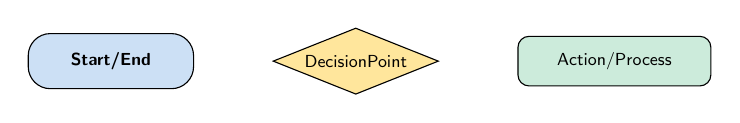
\begin{tikzpicture}[node distance=0.5cm]
\node[startstop, scale=0.7] (start) {Start/End};
\node[decision, right=1cm of start, scale=0.7] (dec) {Decision\\Point};
\node[process, right=1cm of dec, scale=0.7] (proc) {Action/Process};
\end{tikzpicture}
\end{minipage}
\begin{minipage}{0.48\textwidth}
\textbf{Urgency Color Coding:}\\[2pt]
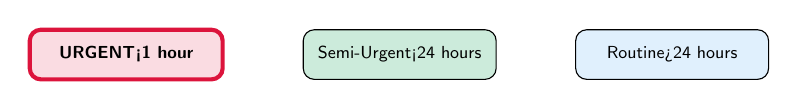
\begin{tikzpicture}[node distance=0.5cm]
\node[urgent, scale=0.7] (urg) {URGENT\\<1 hour};
\node[process, right=1cm of urg, scale=0.7] (sem) {Semi-Urgent\\<24 hours};
\node[routine, right=1cm of sem, scale=0.7] (rout) {Routine\\>24 hours};
\end{tikzpicture}
\end{minipage}
\end{tcolorbox}

\vspace{4pt}

% Main flowchart
\begin{center}
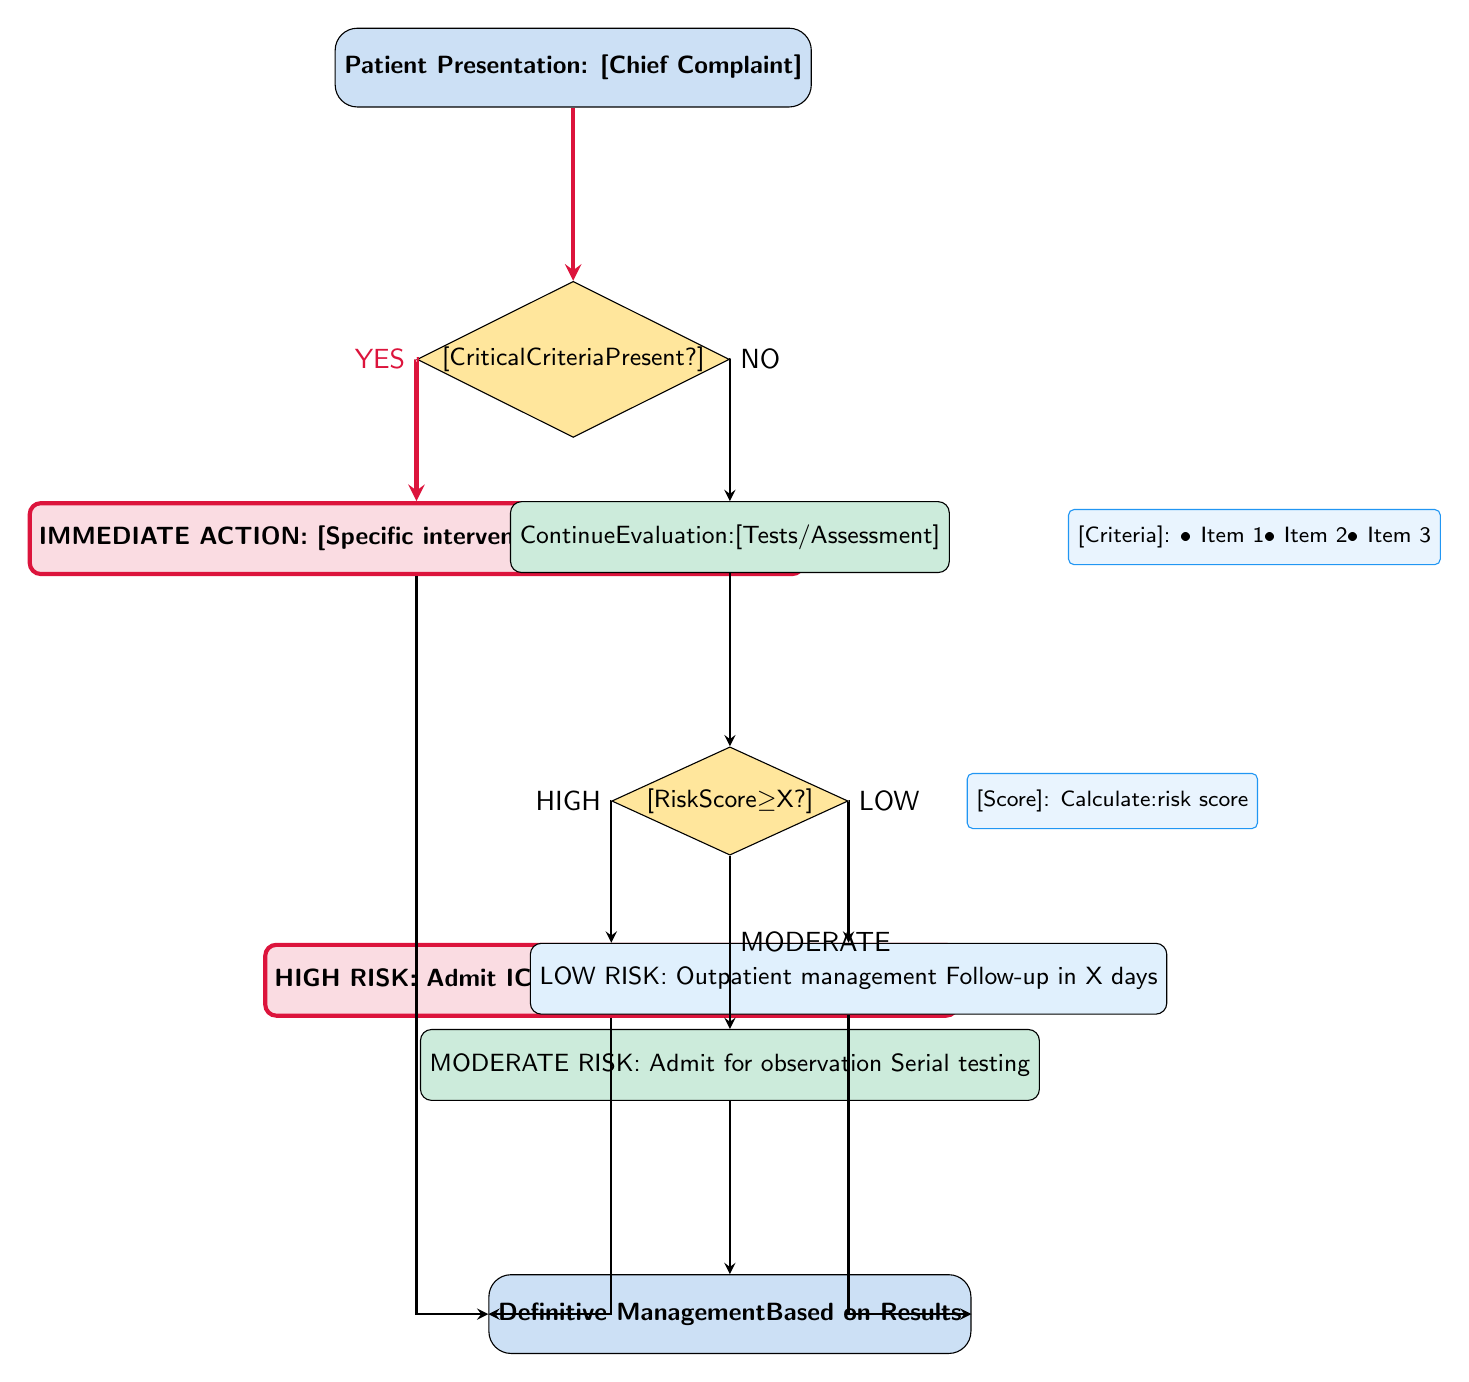
\begin{tikzpicture}[node distance=2.2cm and 3cm, auto]

% Start
\node [startstop] (start) {Patient Presentation:\\[2pt] [Chief Complaint]};

% First decision
\node [decision, below=of start] (decision1) {[Critical\\Criteria\\Present?]};

% Urgent pathway (left branch)
\node [urgent, left=of decision1, below=1.8cm] (urgent1) {IMMEDIATE ACTION:\\[2pt] [Specific intervention]\\[2pt] Call Code/Transfer};

% Continue evaluation (right branch)
\node [process, right=of decision1, below=1.8cm] (eval1) {Continue\\Evaluation:\\[2pt][Tests/Assessment]};

% Second decision
\node [decision, below=of eval1] (decision2) {[Risk\\Score\\$\geq$X?]};

% High risk pathway
\node [urgent, left=of decision2, below=1.8cm] (high) {HIGH RISK:\\[2pt] Admit ICU/Telemetry\\[2pt] [Specific management]};

% Moderate risk
\node [process, below=of decision2] (moderate) {MODERATE RISK:\\[2pt] Admit for observation\\[2pt] Serial testing};

% Low risk pathway
\node [routine, right=of decision2, below=1.8cm] (low) {LOW RISK:\\[2pt] Outpatient management\\[2pt] Follow-up in X days};

% Final outcome node
\node [startstop, below=of moderate, node distance=2.5cm] (outcome) {Definitive Management\\Based on Results};

% Arrows
\draw [urgentarrow] (start) -- (decision1);
\draw [urgentarrow] (decision1) -| node[near start,left] {YES} (urgent1);
\draw [arrow] (decision1) -| node[near start,right] {NO} (eval1);
\draw [arrow] (eval1) -- (decision2);
\draw [arrow] (decision2) -| node[near start,left] {HIGH} (high);
\draw [arrow] (decision2) -- node[right] {MODERATE} (moderate);
\draw [arrow] (decision2) -| node[near start,right] {LOW} (low);
\draw [arrow] (urgent1) |- (outcome);
\draw [arrow] (high) |- (outcome);
\draw [arrow] (moderate) -- (outcome);
\draw [arrow] (low) |- (outcome);

% Information boxes
\node [info, right=1.5cm of eval1] (info1) {[Criteria]:\\[1pt] \footnotesize • Item 1\\• Item 2\\• Item 3};
\node [info, right=1.5cm of decision2] (info2) {[Score]:\\[1pt] \footnotesize Calculate:\\risk score};

\end{tikzpicture}
\end{center}

\vspace{8pt}

% Detailed pathway steps
\begin{tcolorbox}[colback=highlightgray!30,colframe=headerblue,title=\textbf{Detailed Pathway Steps},fonttitle=\bfseries]

\textbf{STEP 1: Initial Assessment}
\begin{itemize}
\item Vital signs: BP, HR, RR, temp, O₂ saturation
\item Focused history: [Key elements]
\item Physical examination: [Key findings]
\item Initial labs: [Specify tests]
\item ECG (if applicable)
\end{itemize}

\textbf{STEP 2: Risk Stratification}
\begin{itemize}
\item Calculate [Risk Score Name] (see scoring table below)
\item Identify high-risk features requiring immediate intervention
\item Document risk category in medical record
\end{itemize}

\textbf{STEP 3: Treatment Initiation}
\begin{itemize}
\item Urgent: [Specific interventions within 1 hour]
\item Semi-urgent: [Interventions within 24 hours]
\item Routine: [Standard management approach]
\end{itemize}

\textbf{STEP 4: Monitoring and Reassessment}
\begin{itemize}
\item Frequency: [Based on risk category]
\item Parameters: [What to monitor]
\item Escalation criteria: [When to intensify treatment]
\item De-escalation criteria: [When to transition to lower intensity]
\end{itemize}

\end{tcolorbox}

\vspace{4pt}

% Risk scoring table
\begin{tcolorbox}[colback=white,colframe=headerblue,title=\textbf{[Risk Score Name] Calculation},fonttitle=\bfseries]
{\small
\begin{tabular}{lc}
\toprule
\textbf{Clinical Feature} & \textbf{Points} \\
\midrule
[Feature 1 - e.g., Age $\geq$65 years] & +1 \\
[Feature 2 - e.g., Prior history] & +1 \\
[Feature 3 - e.g., Abnormal lab value] & +2 \\
[Feature 4 - e.g., Specific symptom] & +1 \\
[Feature 5 - e.g., Imaging finding] & +2 \\
\midrule
\textbf{Total Score} & \textbf{0-X points} \\
\bottomrule
\end{tabular}

\vspace{4pt}

\textbf{Risk Categories}:
\begin{itemize}
\item \textbf{Low Risk}: 0-1 points → [Management approach, predicted outcome]
\item \textbf{Moderate Risk}: 2-3 points → [Management approach, predicted outcome]
\item \textbf{High Risk}: $\geq$4 points → [Management approach, predicted outcome]
\end{itemize}
}
\end{tcolorbox}

\vspace{4pt}

% Evidence basis
\begin{tcolorbox}[colback=actiongreen!5,colframe=actiongreen,title=\textbf{Evidence Basis for Pathway},fonttitle=\bfseries]
{\small
\textbf{Key Supporting Evidence}:
\begin{enumerate}
\item \textbf{[Clinical Trial/Study]}: [Key finding supporting pathway decision]
\item \textbf{Guidelines}: NCCN/ASCO/AHA/ACC/[Relevant society] [Year] - [Recommendation level]
\item \textbf{Meta-Analysis}: [If applicable - pooled results supporting approach]
\end{enumerate}

\textbf{Validation}: Pathway validated at [institution] with [X\%] adherence rate and [outcome metrics].

\textbf{Last Updated}: [Date] based on [new trial, guideline update, or scheduled review]
}
\end{tcolorbox}

\vspace{8pt}

\hrule
\vspace{4pt}
{\footnotesize
\textbf{Pathway Committee}: [Names, titles] | \textbf{Approved}: [Date] | \textbf{Next Review}: [Date]\\
\textbf{Contact for Questions}: [Name, email, phone]
}

\end{document}

